\documentclass[journal,a4paper]{IEEEtran}
\IEEEoverridecommandlockouts
\usepackage{cite}
\usepackage{amsmath,amssymb,amsfonts}
\usepackage{algorithmic}
\usepackage{graphicx}
\usepackage{textcomp}
\usepackage{xcolor}
\usepackage{booktabs}
\usepackage{algorithm}
\usepackage{float}
\usepackage{microtype} 
% Proper IEEE Captions: Centered, 8pt font, and Table titles in Small Caps
\usepackage[font=footnotesize,justification=centering]{caption}
\DeclareCaptionLabelSeparator{periodspace}{. }
\captionsetup{labelsep=periodspace}

% Symbol rendering
\usepackage{textcomp}
\newcommand{\peso}{{\textpeso}}

\def\BibTeX{{\rm B\kern-.05em{\sc i\kern-.025em b}\kern-.08em
    T\kern-.1667em\lower.7ex\hbox{E}\kern-.125emX}}

\begin{document}

\title{Adaptive Policy Optimization for Municipal Solid Waste Segregation using Coupled Agent-Based Modeling and Deep Reinforcement Learning}

\author{
\IEEEauthorblockN{Jemar John J. Lumingkit, Hussam M. Bansao, and Dante D. Dinawanao} \\
\IEEEauthorblockA{\textit{Department of Computer Science,}
\textit{Mindanao State University - Iligan Institute of Technology}\\
Iligan City, Philippines \\
\{jemarjohn.lumingkit, hussam.bansao, dante.dinawanao\}@g.msuiit.edu.ph}
}

\maketitle

\begin{abstract}
Achieving a resilient and sustainable society requires intelligent systems capable of navigating the complex behavioral dynamics of urban waste management. The "MRF Paradox" exposes a systemic failure in this transition: nationwide increases in Material Recovery Facilities (MRFs) often coincide with simultaneous surges in illegal dumping. This suggests that infrastructure alone is insufficient; the fundamental bottleneck lies within household-level behavioral friction. We introduce an intelligent framework coupling an Agent-Based Model (ABM) with a Heuristic-Guided Deep Reinforcement Learning (HuDRL) agent. Formalizing household cognition via the Theory of Planned Behavior, sensitivity analysis proves that internal household friction drives 79\% of non-compliance. Our HuDRL agent discovers a "Sequential Saturation" strategy to trigger localized social tipping points. This research provides a predictive paradigm for resilient municipal governance, transforming trial-and-error budgeting into a defensible, data-driven system for sustainable environmental outcomes.
\end{abstract}

\begin{IEEEkeywords}
Agent-Based Modeling, Deep Reinforcement Learning, Municipal Solid Waste Management, Polycentric Governance, Resilient Systems.
\end{IEEEkeywords}

\section{Introduction}
Building a resilient and sustainable society necessitates a fundamental shift in how municipalities manage solid waste (MSW). In the Philippines, the implementation of R.A. 9003 has encountered the "MRF Paradox": despite a surge in mandated Material Recovery Facilities (MRFs), illegal dumping and non-compliance continue to escalate. This paradox highlights that physical infrastructure alone cannot overcome deeply ingrained behavioral inertia. The true bottleneck is the internal friction of household-level labor—washing, sorting, and storing waste—which currently traps Local Government Units (LGUs) in a cycle of trial-and-error budgeting.

Optimizing policy in these environments is a high-dimensional systems analysis challenge characterized by human hysteresis~\cite{tian2024}. Psychological models like the Theory of Planned Behavior (TPB) clarify that intentions are frequently overridden by the physical "Cost of Effort"~\cite{taraghi2025, moeini2023}. While Deep Reinforcement Learning (DRL) offers a path to autonomous policy discovery~\cite{zheng2022b}, standard agents suffer from a severe "Sparse Reward Problem." They struggle to link short-term fiscal actions to the long-term, sustained pressure required to reach critical social tipping points~\cite{centola2018, andre2021}.

To foster resilient municipal governance, this study proposes an intelligent system coupling an ABM with a Heuristic-Guided DRL (HuDRL) agent. By simulating household friction and neighborhood influence, the HuDRL agent navigates a non-convex policy space to discover budget allocations that maximize long-term compliance. This methodology provides LGUs with a mathematical foundation to transition from reactive spending to a predictive framework for sustainable development.

\section{Related Work}
Sustainable waste management depends on the "Intention-Action Gap." Psychological research indicates that even with high environmental awareness, participation drops as the physical labor of sorting increases~\cite{moeini2023}. Ceschi et al.~\cite{ceschi} utilized ABM to nudge recycling behavior through norm-based policies, demonstrating that peer influence is a critical driver of adoption. Furthermore, the "AI Economist" established the efficacy of utilizing multi-agent reinforcement learning to optimize high-dimensional policy spaces like taxation~\cite{zheng2022b}. This study builds upon these foundations by applying DRL to the socio-technical challenge of inducing source segregation within a polycentric governance structure.

\section{System Architecture and Environment}
The simulation is geographically bounded to Bacolod, Lanao del Norte. It utilizes a spatially explicit $50 \times 50$ grid containing 4,022 Household Agents across seven barangays. The architecture bridges micro-behavior and macro-policy via a dual-clock resolution: households execute logic on daily ticks, while the central Mayor Agent executes budget distributions on quarterly (90-day) epochs over a 3-year simulation horizon. Meso-level Barangay Agents act as data aggregators, compressing micro-outputs into 17-dimensional state vectors.

\begin{figure}[htbp] 
\centering
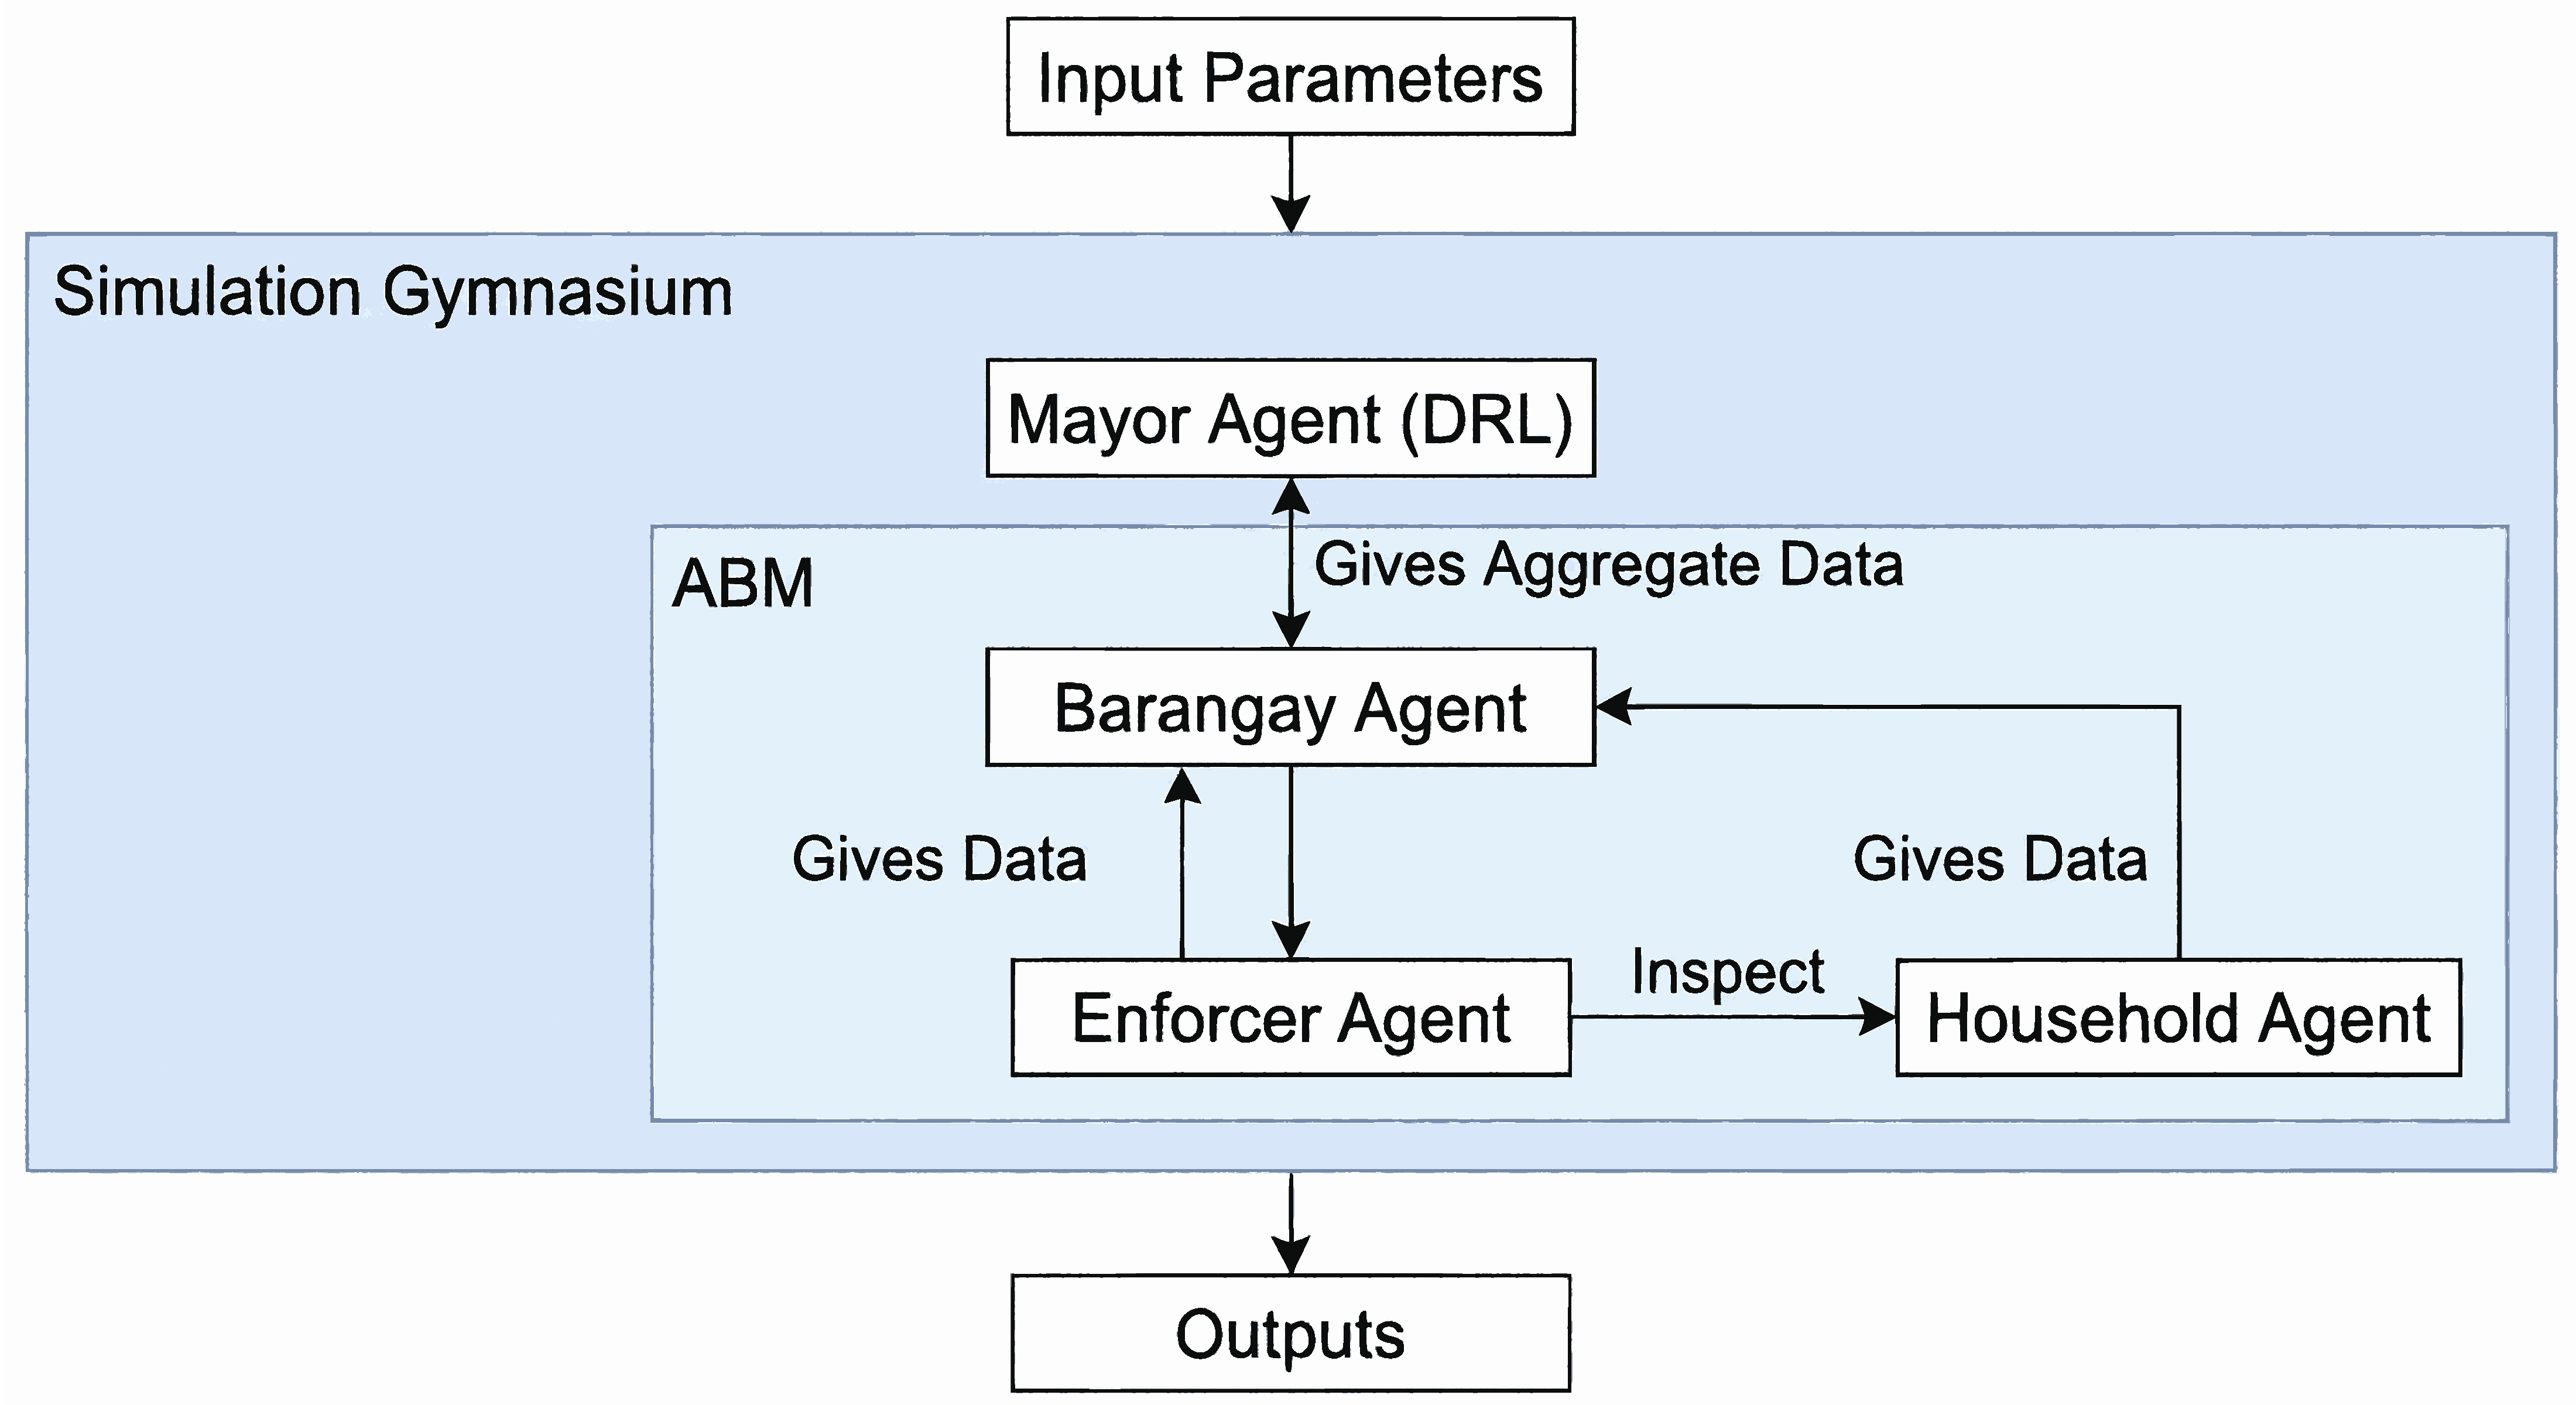
\includegraphics[width=0.85\columnwidth]{images/simul_gym.pdf}
\caption{System Architecture. The diagram illustrates the coupling between the ABM micro-simulation and the HuDRL macro-optimization agent.}
\label{fig:simul_diagram}
\end{figure}

\section{Multi-Agent Modeling}
\subsection{Household Cognition and Structural Friction}
Household behavior is governed by a dynamically weighted TPB utility equation ($U_{seg}$) derived from Ceschi et al.~\cite{ceschi}:
\begin{equation}
U_{seg} = (w_{A}A) + (w_{SN}SN_{loc}) + (w_{PBC}PBC) - C_{Net} + \epsilon
\end{equation}
The Net Cost ($C_{Net}$) function mathematically formalizes structural friction:
\begin{equation}
    C_{Net} = C_{Effort} + \eta (C_{Mon} - I - F \cdot P_{Detect})
\end{equation}
where $C_{Effort}$ is the internal friction of household labor and $\eta$ is the income-sensitivity multiplier. To model cultural resilience, if local compliance breaches the 70\% tipping point ($SN_{loc} \ge 0.70$), the behavior internalizes, creating a "Social Norm Shield" where the behavior resists decay even if incentives are removed.

\section{The HuDRL Optimization Framework}

\subsection{MDP Specification}
The policymaker is formalized as an episodic MDP defined by $\langle \mathcal{S}, \mathcal{A}, \mathcal{P}, \mathcal{R}, \gamma \rangle$. To ensure technical rigor, the state and action spaces are detailed in Table~\ref{tab:mdp}.

\begin{table}[htbp]
\centering
\caption{MDP State and Action Space Definitions}
\label{tab:mdp}
\footnotesize
\begin{tabular}{lp{5.5cm}}
\toprule
Space & Components \\
\midrule
\textbf{State ($\mathcal{S}$)} & Quarterly compliance per barangay ($\times7$), budget exhaustion rates ($\times7$), global compliance, quarter index, political capital. \\
\textbf{Action ($\mathcal{A}$)} & Continuous vector representing funding for IEC, Enforcement, and Incentives across 7 barangays (21 dimensions). \\
\bottomrule
\end{tabular}
\end{table}

\subsection{Action Masking and Training Setup}
To navigate the non-convex policy space, we utilize a 70\% Graduation Mechanism. Once a locale hits the tipping point, the algorithm slashes funding by 99\%, forcing the agent to pivot resources to failing areas. The agent was trained using PPO with the configuration in Table~\ref{tab:hyperparameters}.

\begin{table}[htbp]
\centering
\caption{PPO Training Configuration and Hyperparameters}
\label{tab:hyperparameters}
\footnotesize
\begin{tabular}{ll}
\toprule
Parameter & Value \\
\midrule
Parallel Environments & 4 (SubprocVecEnv) \\
Rollout Buffer ($n\_steps$) & 1,024 \\
Batch Size & 128 \\
Learning Rate & $3 \times 10^{-4}$ \\
Entropy Coefficient & 0.01 \\
Total Timesteps & 500,000 \\
Evaluation Metric & Mean $\pm$ Std (5 random seeds) \\
\bottomrule
\end{tabular}
\end{table}

\section{Results and Discussion}

\subsection{Global Sensitivity Analysis}
Sobol Global Sensitivity Analysis ($N=1024$) proves that $C_{effort}$ is the dominant driver of the MRF Paradox, accounting for 79.2\% of system variance (Table~\ref{tab:sobol}).

\begin{table}[htbp]
\centering
\caption{Sobol Indices for Household Compliance Factors}
\label{tab:sobol}
\footnotesize
\begin{tabular}{lcccc}
\toprule
Factor & $S_1$ & $S_T$ & 95\% CI & Total Var. \\
\midrule
Cost of Effort ($C_{Effort}$) & 0.792 & 0.841 & $\pm$0.038 & 79.2\% \\
Perceived Behavioral Control ($w_{PBC}$) & 0.081 & 0.114 & $\pm$0.012 & 8.1\% \\
Social Norms ($w_{SN}$) & 0.045 & 0.062 & $\pm$0.009 & 4.5\% \\
Decay Rate ($k_{decay}$) & 0.024 & 0.038 & $\pm$0.006 & 2.4\% \\
Attitude Weight ($w_{A}$) & 0.014 & 0.028 & $\pm$0.004 & 1.4\% \\
\bottomrule
\end{tabular}
\end{table}

\subsection{Policy Traps and Zones}
We numerically define several observed states:
\begin{itemize}
    \item \textbf{Collapse Zone:} Sustained compliance $<25\%$ across all barangays for $\ge3$ consecutive quarters.
    \item \textbf{Draconian Trap:} Spiking enforcement causing \textit{Political Collapse} (approval $<10\%$), leading to administrative failure.
    \item \textbf{Transactional Trap:} Budget exhaustion without established norms, where compliance drops immediately upon incentive withdrawal.
\end{itemize}

\subsection{Comparative Analysis of Policy Strategies}
Simulation experiments demonstrate a stark divergence between intuitive heuristics and DRL optimization (Table~\ref{tab:results}). The \textit{Status Quo} baseline distributing funds equally created an "Urban Resource Trap" in dense areas. The HuDRL agent’s discovery of \textit{"Sequential Saturation"}—concentrating up to 69\% of budget on single failing nodes—proves that resolving the MRF Paradox requires bypassing human bias toward simultaneous fairness.

\begin{table}[htbp]
\centering
\caption{Compliance Rates of Simulated Policy Strategies}
\label{tab:results}
\footnotesize
\begin{tabular}{ll}
\toprule
Policy Strategy & Global Compliance (\%) \\
\midrule
Status Quo (Equitable Distribution) & 30.18\% \\
Pure Enforcement & Political Collapse (Q2) \\
Pure Incentives & 15.91\% \\
\textbf{HuDRL (Proposed)} & \textbf{90.45\%} \\
\bottomrule
\end{tabular}
\end{table}

\begin{figure}[htbp] 
    \centering
    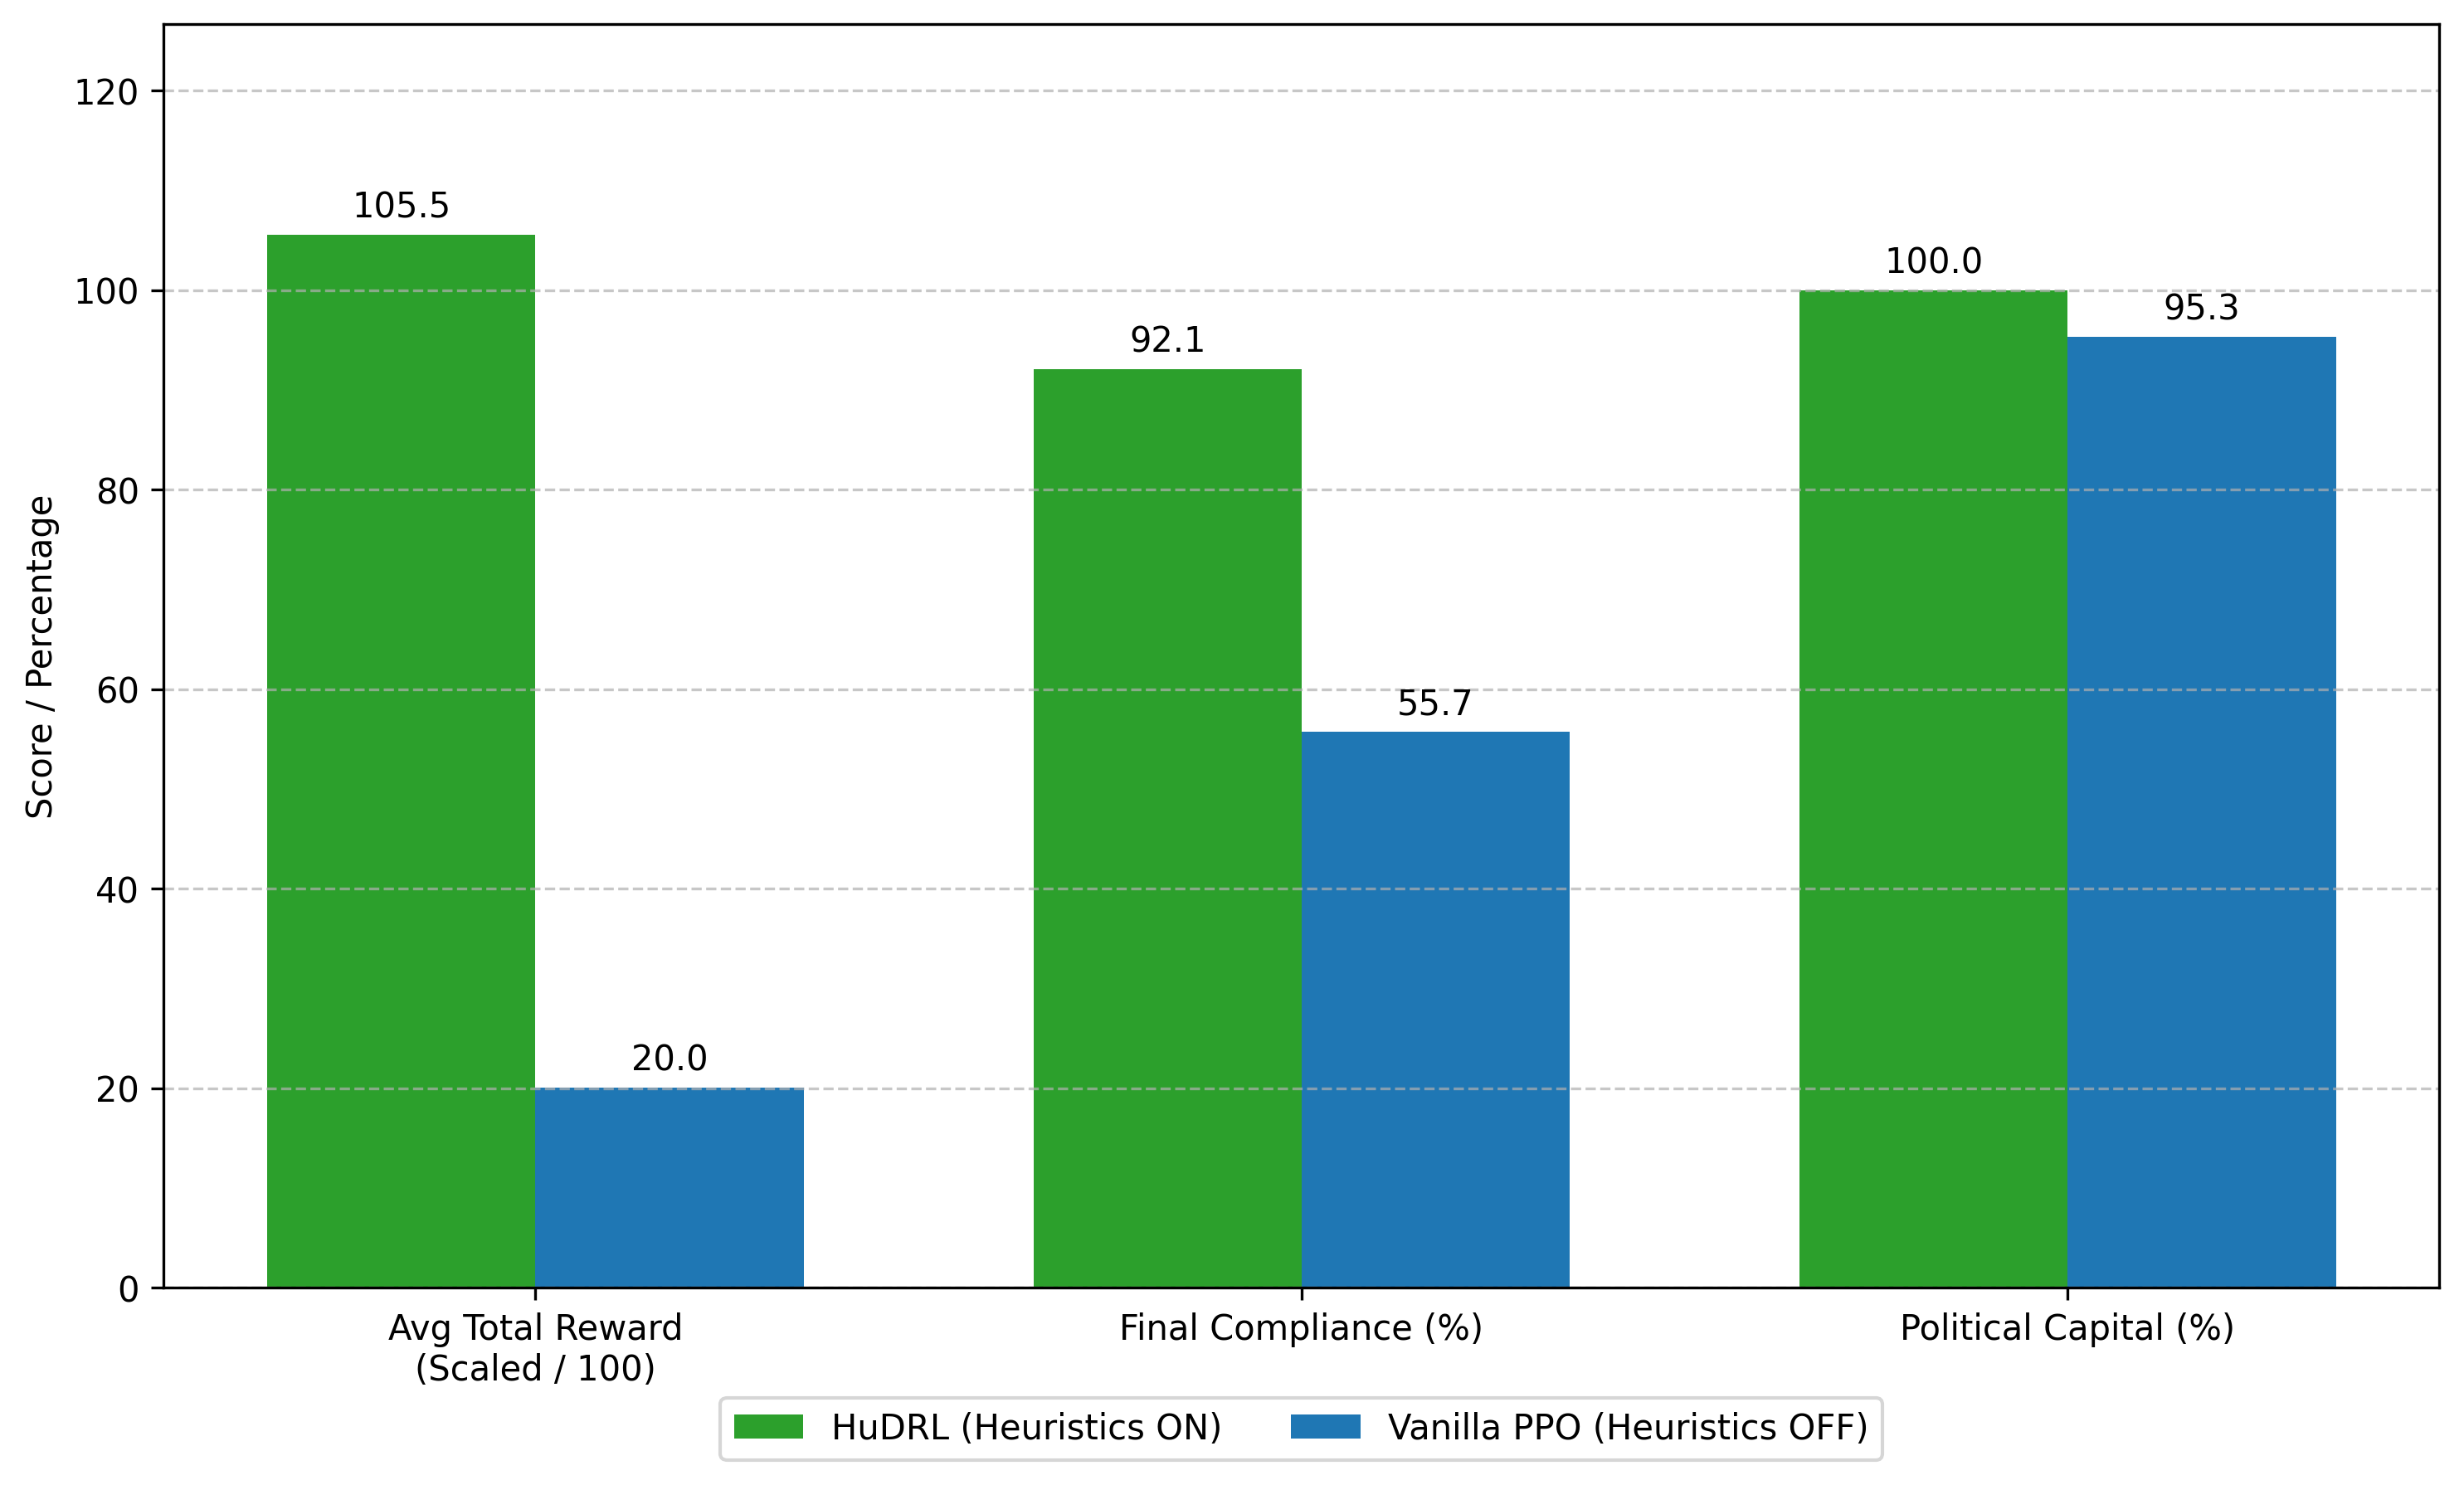
\includegraphics[width=0.85\columnwidth]{images/hudrl_vs_vanilla.png}
    \caption{Convergence Profile. HuDRL crosses the stability threshold by Q2, whereas standard PPO remains in the Collapse Zone.}
\label{fig:convergence}
\end{figure}

\section{Conclusion and Recommendations}
This study proves that resolving the "MRF Paradox" requires a shift from infrastructure-centric management to a \textit{Sequential Saturation} model. We recommend that LGUs concentrate resources on specific barangays to trigger tipping points before pivoting. Additionally, policy should prioritize reducing household "Cost of Effort" (e.g., providing pre-labeled bins) to maximize long-term environmental sustainability.

\section*{Acknowledgment}
The authors thank the LGU of Bacolod and MSU-IIT for their support. This work received no external funding. Reproducibility: Code at [GitHub/Zenodo].

\section*{Use of Generative AI}
The authors used Google Gemini Pro for language refinement (grammar, phrasing, and readability) across the Abstract, Introduction, and Conclusion. The AI system did not contribute to research design or results interpretation.

\begin{thebibliography}{00}
\footnotesize
\bibitem{ra9003} Republic of the Philippines, ``Ecological Solid Waste Management Act of 2000, Rep. Act No. 9003,'' Jan. 2001.
\bibitem{tian2024} X. Tian, et al., ``Agent-based modeling in solid waste management,'' \textit{Env. Impact Assess. Rev.}, vol. 110, 2024.
\bibitem{centola2018} D. Centola, et al., ``Experimental evidence for tipping points in social convention,'' \textit{Science}, vol. 360, 2018.
\bibitem{taraghi2025} M. Taraghi and L. Yoder, ``Integrating the theory of planned behavior in ABMs,'' \textit{Ecological Modelling}, vol. 508, 2025.
\bibitem{moeini2023} B. Moeini, et al., ``Effect of household interventions on promoting waste segregation,'' \textit{Sustainability}, vol. 15, 2023.
\bibitem{zheng2022b} S. Zheng, et al., ``The AI Economist: Taxation policy design via RL,'' \textit{Science Advances}, vol. 8, no. 18, 2022.
\bibitem{ceschi} A. Ceschi, et al., ``Testing a norm-based policy for waste management,'' \textit{Journal of Env. Mgmt.}, vol. 294, 2021.
\end{thebibliography}

\end{document}